\documentclass{standalone}
\usepackage{tikz}
\usetikzlibrary{patterns, positioning}
\usepackage[sfdefault]{ClearSans} %% option 'sfdefault' activates Clear Sans as the default text font
\usepackage[T1]{fontenc}

\begin{document}
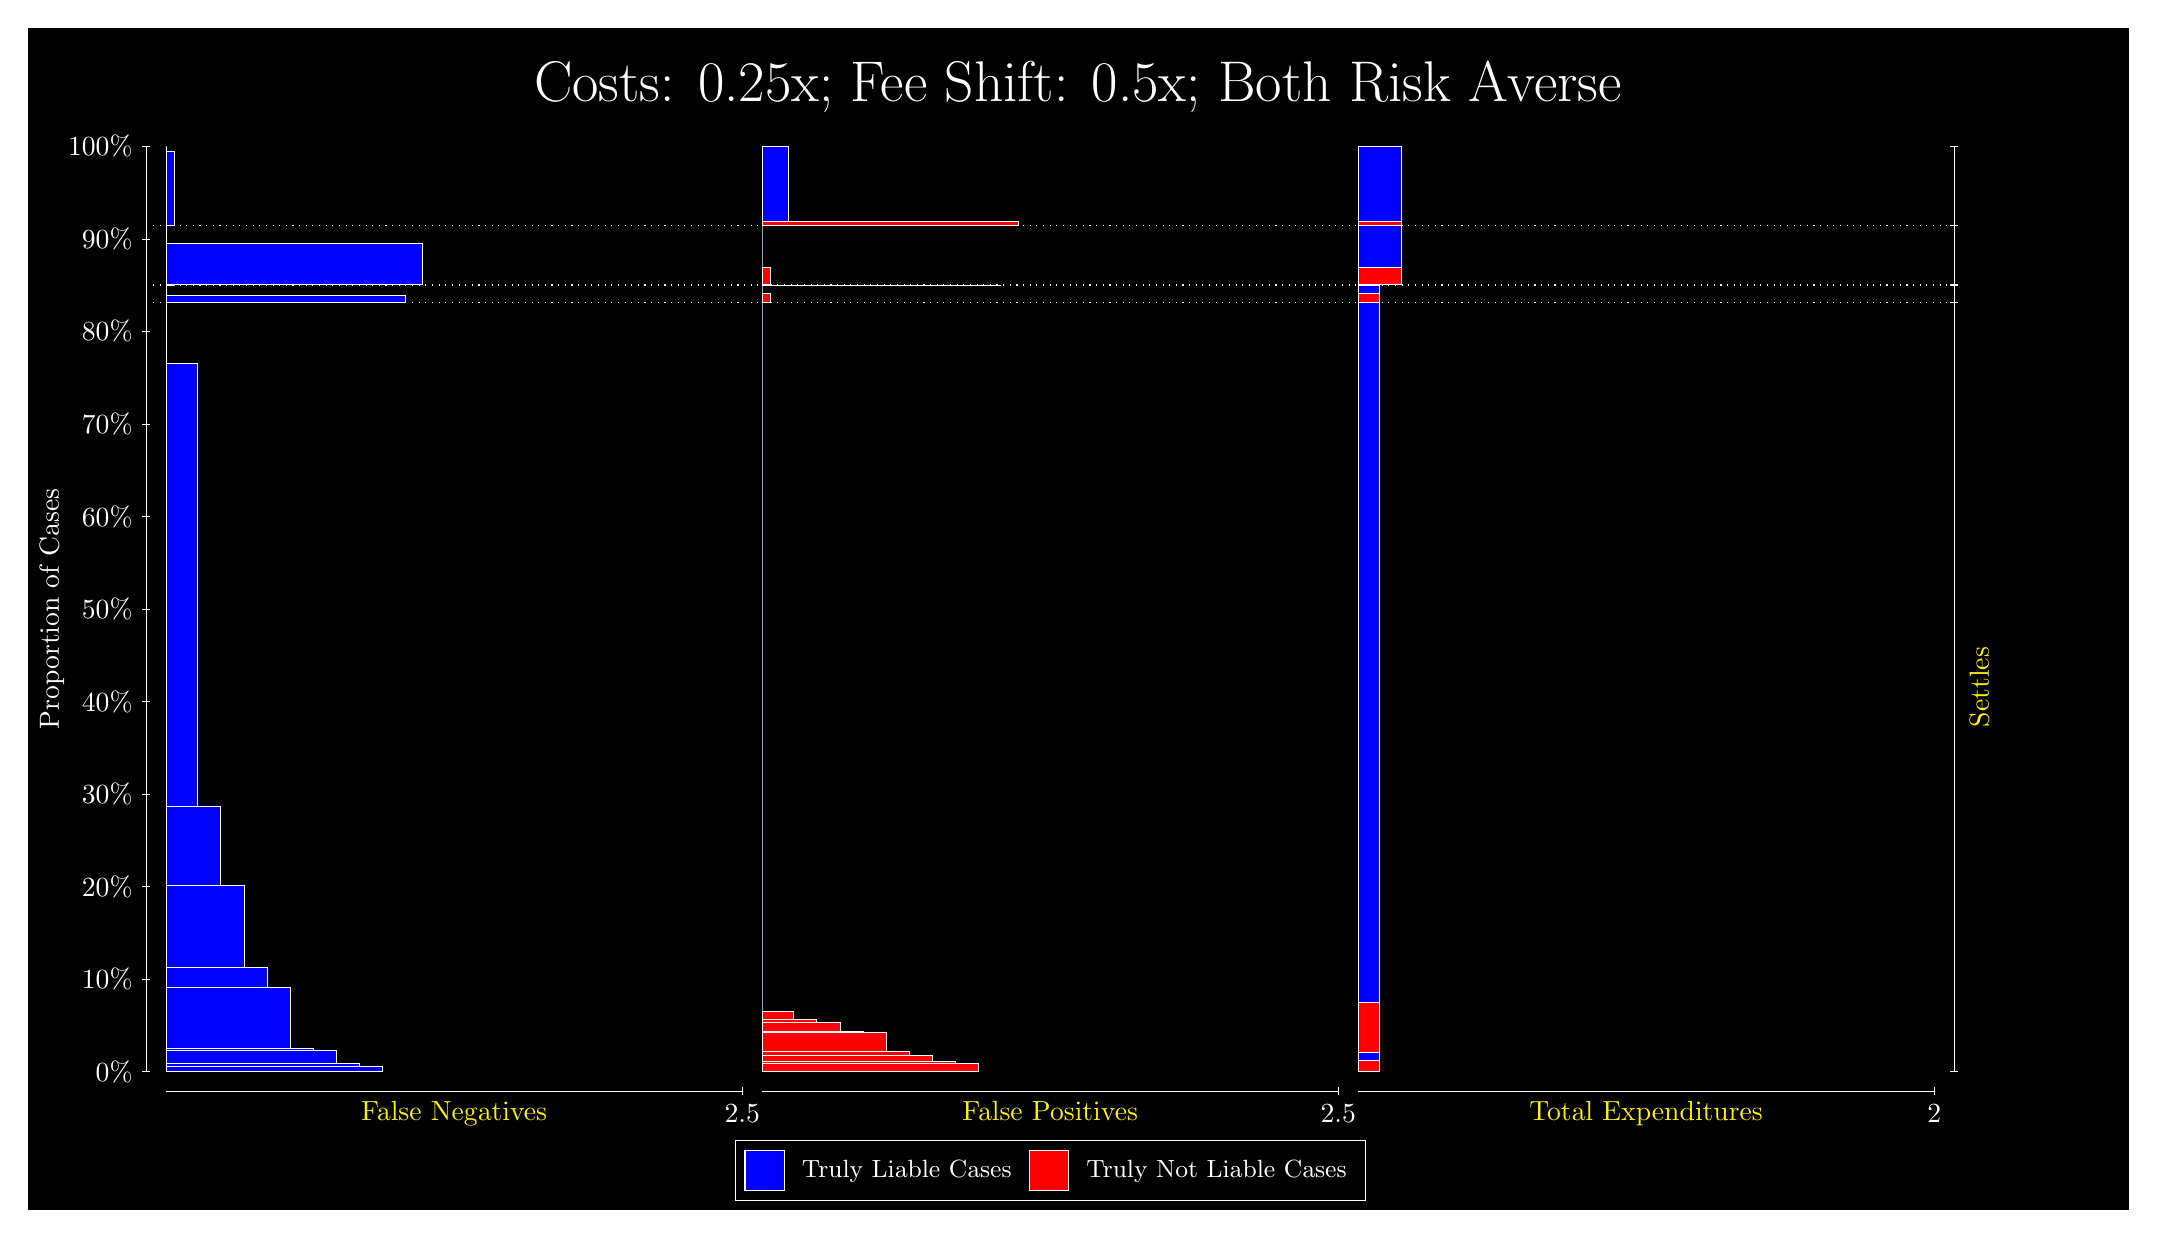
\begin{tikzpicture}
\draw[fill=black] (0,0) rectangle (26.667,15);
\draw[text=white] (0,13.5) rectangle (26.667,15) node[midway] {\huge Costs: 0.25x; Fee Shift: 0.5x; Both Risk Averse};
\draw[white, very thin] (1.5,1.75) -- (1.5,13.5);
\node[rotate=90, text=white, anchor=center] at (0.3, 7.625) {Proportion of Cases};
\draw[white, very thin] (1.45,1.75) -- (1.55,1.75);
\node[text=white, anchor=east] at (1.45, 1.75) {0\%};
\draw[white, very thin] (1.45,2.925) -- (1.55,2.925);
\node[text=white, anchor=east] at (1.45, 2.925) {10\%};
\draw[white, very thin] (1.45,4.1) -- (1.55,4.1);
\node[text=white, anchor=east] at (1.45, 4.1) {20\%};
\draw[white, very thin] (1.45,5.275) -- (1.55,5.275);
\node[text=white, anchor=east] at (1.45, 5.275) {30\%};
\draw[white, very thin] (1.45,6.45) -- (1.55,6.45);
\node[text=white, anchor=east] at (1.45, 6.45) {40\%};
\draw[white, very thin] (1.45,7.625) -- (1.55,7.625);
\node[text=white, anchor=east] at (1.45, 7.625) {50\%};
\draw[white, very thin] (1.45,8.8) -- (1.55,8.8);
\node[text=white, anchor=east] at (1.45, 8.8) {60\%};
\draw[white, very thin] (1.45,9.975) -- (1.55,9.975);
\node[text=white, anchor=east] at (1.45, 9.975) {70\%};
\draw[white, very thin] (1.45,11.15) -- (1.55,11.15);
\node[text=white, anchor=east] at (1.45, 11.15) {80\%};
\draw[white, very thin] (1.45,12.325) -- (1.55,12.325);
\node[text=white, anchor=east] at (1.45, 12.325) {90\%};
\draw[white, very thin] (1.45,13.5) -- (1.55,13.5);
\node[text=white, anchor=east] at (1.45, 13.5) {100\%};

\draw[white, very thin] (24.457,1.75) -- (24.457,13.5);
\draw[white, very thin] (24.407,1.75) -- (24.507,1.75);
\node[anchor=west] at (24.407, 1.75) {};
\draw[white, very thin] (24.407,11.514) -- (24.507,11.514);
\node[anchor=west] at (24.407, 11.514) {};
\draw[white, very thin] (24.407,11.736) -- (24.507,11.736);
\node[anchor=west] at (24.407, 11.736) {};
\draw[white, very thin] (24.407,11.743) -- (24.507,11.743);
\node[anchor=west] at (24.407, 11.743) {};
\draw[white, very thin] (24.407,12.491) -- (24.507,12.491);
\node[anchor=west] at (24.407, 12.491) {};
\draw[white, very thin] (24.407,13.5) -- (24.507,13.5);
\node[anchor=west] at (24.407, 13.5) {};

\draw[white, very thin, fill=blue] (1.75,1.75) rectangle (4.4946,1.8215);
\draw[white, very thin, fill=blue] (1.75,1.8215) rectangle (4.2018,1.8566);
\draw[white, very thin, fill=blue] (1.75,1.8566) rectangle (3.9091,2.0146);
\draw[white, very thin, fill=blue] (1.75,2.0146) rectangle (3.6163,2.044);
\draw[white, very thin, fill=blue] (1.75,2.044) rectangle (3.3236,2.8185);
\draw[white, very thin, fill=blue] (1.75,2.8185) rectangle (3.0308,3.0728);
\draw[white, very thin, fill=blue] (1.75,3.0728) rectangle (2.738,4.1187);
\draw[white, very thin, fill=blue] (1.75,4.1187) rectangle (2.4453,5.1249);
\draw[white, very thin, fill=blue] (1.75,5.1249) rectangle (2.1525,10.744);
\draw[white, very thin, fill=red] (1.75,10.744) rectangle (1.75,11.514);
\draw[white, very thin, fill=blue] (1.75,11.514) rectangle (4.7873,11.611);
\draw[white, very thin, fill=red] (1.75,11.611) rectangle (1.75,11.736);
\draw[white, very thin, fill=blue] (1.75,11.736) rectangle (1.8598,11.743);
\draw[white, very thin, fill=red] (1.75,11.743) rectangle (1.75,11.743);
\draw[white, very thin, fill=blue] (1.75,11.743) rectangle (5.0069,12.27);
\draw[white, very thin, fill=red] (1.75,12.27) rectangle (1.75,12.491);
\draw[white, very thin, fill=blue] (1.75,12.491) rectangle (1.8598,13.442);
\draw[white, very thin, fill=red] (1.75,13.442) rectangle (1.75,13.5);
\draw[white, very thin, fill=red] (9.3189,1.75) rectangle (12.063,1.8548);
\draw[white, very thin, fill=red] (9.3189,1.8548) rectangle (11.771,1.8832);
\draw[white, very thin, fill=red] (9.3189,1.8832) rectangle (11.478,1.9589);
\draw[white, very thin, fill=red] (9.3189,1.9589) rectangle (11.185,2.0032);
\draw[white, very thin, fill=red] (9.3189,2.0032) rectangle (10.892,2.2454);
\draw[white, very thin, fill=red] (9.3189,2.2454) rectangle (10.6,2.2609);
\draw[white, very thin, fill=red] (9.3189,2.2609) rectangle (10.307,2.3818);
\draw[white, very thin, fill=red] (9.3189,2.3818) rectangle (10.014,2.4178);
\draw[white, very thin, fill=red] (9.3189,2.4178) rectangle (9.7214,2.5203);
\draw[white, very thin, fill=blue] (9.3189,2.5203) rectangle (9.3189,11.514);
\draw[white, very thin, fill=red] (9.3189,11.514) rectangle (9.4287,11.639);
\draw[white, very thin, fill=blue] (9.3189,11.639) rectangle (9.3189,11.736);
\draw[white, very thin, fill=red] (9.3189,11.736) rectangle (12.356,11.736);
\draw[white, very thin, fill=blue] (9.3189,11.736) rectangle (9.4287,11.743);
\draw[white, very thin, fill=red] (9.3189,11.743) rectangle (9.4287,11.964);
\draw[white, very thin, fill=blue] (9.3189,11.964) rectangle (9.3189,12.491);
\draw[white, very thin, fill=red] (9.3189,12.491) rectangle (12.576,12.549);
\draw[white, very thin, fill=blue] (9.3189,12.549) rectangle (9.6482,13.5);
\draw[white, very thin, fill=red] (16.888,1.75) rectangle (17.162,1.8886);
\draw[white, very thin, fill=blue] (16.888,1.8886) rectangle (17.162,1.9951);
\draw[white, very thin, fill=red] (16.888,1.9951) rectangle (17.162,2.6269);
\draw[white, very thin, fill=blue] (16.888,2.6269) rectangle (17.162,11.514);
\draw[white, very thin, fill=red] (16.888,11.514) rectangle (17.162,11.639);
\draw[white, very thin, fill=blue] (16.888,11.639) rectangle (17.162,11.736);
\draw[white, very thin, fill=red] (16.888,11.736) rectangle (17.162,11.736);
\draw[white, very thin, fill=blue] (16.888,11.736) rectangle (17.162,11.743);
\draw[white, very thin, fill=red] (16.888,11.743) rectangle (17.437,11.964);
\draw[white, very thin, fill=blue] (16.888,11.964) rectangle (17.437,12.491);
\draw[white, very thin, fill=red] (16.888,12.491) rectangle (17.437,12.549);
\draw[white, very thin, fill=blue] (16.888,12.549) rectangle (17.437,13.5);
\draw[white, dotted] (1.5,11.514) -- (24.457,11.514);
\draw[white, dotted] (1.5,11.736) -- (24.457,11.736);
\draw[white, dotted] (1.5,11.743) -- (24.457,11.743);
\draw[white, dotted] (1.5,12.491) -- (24.457,12.491);
\draw[white, very thin] (1.75,1.5) -- (9.0689,1.5);
\node[text=yellow, anchor=north] at (5.4094, 1.5) {False Negatives};
\draw[white, very thin] (9.0689,1.45) -- (9.0689,1.55);
\node[text=white, anchor=north] at (9.0689, 1.45) {2.5};

\draw[white, very thin] (9.3189,1.5) -- (16.638,1.5);
\node[text=yellow, anchor=north] at (12.978, 1.5) {False Positives};
\draw[white, very thin] (16.638,1.45) -- (16.638,1.55);
\node[text=white, anchor=north] at (16.638, 1.45) {2.5};

\draw[white, very thin] (16.888,1.5) -- (24.207,1.5);
\node[text=yellow, anchor=north] at (20.547, 1.5) {Total Expenditures};
\draw[white, very thin] (24.207,1.45) -- (24.207,1.55);
\node[text=white, anchor=north] at (24.207, 1.45) {2};

\node[text=yellow, centered, rotate=90] at (24.777, 6.6319) {Settles};





\draw (12.978300999999998,1.5) node[draw=none] (baseCoordinate) {};
\begin{scope}[align=center]
        \matrix[scale=0.5, draw=white, below=0.5cm of baseCoordinate, nodes={draw}, column sep=0.1cm]{
            \node[rectangle, draw, minimum width=0.5cm, minimum height=0.5cm, fill=blue] {}; &
            \node[draw=none, font=\small, text=white] (B) {Truly Liable Cases}; &
            \node[rectangle, draw, minimum width=0.5cm, minimum height=0.5cm, fill=red] {}; &
            \node[draw=none, font=\small, text=white] (B) {Truly Not Liable Cases}; \\
            };
\end{scope}

\end{tikzpicture}
\end{document}